% Especificaciones del tamaño de letra, tamaño de hoja, márgenes, librerias, etc.
\documentclass[12pt, letterpaper]{article}
\usepackage[english]{babel}
\usepackage{fancyhdr}
\usepackage[utf8]{inputenc}
\usepackage[T1]{fontenc}
\usepackage{amsmath}
\usepackage{graphicx}
\usepackage{subcaption}
\usepackage[hidelinks]{hyperref}
\usepackage{url}
\usepackage{amssymb}
\usepackage{float}
\usepackage[margin=1in]{geometry}
\usepackage{listings}
\usepackage{verbatim}
\usepackage[most]{tcolorbox} % Produces color boxes.
\renewcommand{\baselinestretch}{1.5}

\lstset{numbers=left}
% Enlace Bibliografía
\usepackage{csquotes}
\usepackage[notes,backend=biber]{biblatex-chicago}
\addbibresource{referencias.bib}

% Titulo, autores, fecha.
\title{Práctica \#5: Discretización Geométrica (Mallado)}
\author{Carlos A. Vásquez Castañeda \and 1155057 \and Grupo 395}
\date{Marzo 28, 2020}
\pagestyle{fancy}
\fancyhf{}
\rhead{Mecánica de Sustentación}
\lhead{Práctica \#5}
\rfoot{\thepage}

\definecolor{lightgreen}{RGB}{255, 128, 159}
% Inicio del documento
\begin{document}
\maketitle

\section*{Introducción}
El mundo real presenta formas geométricas y objetos bastante complejos. Es sencillo aproximar algunos objetos a paralelepípedos o esferas, sin embargo casi todos los objetos tienen formas irregulares que no se ajustan a la superposición de estos objetos más fáciles de analizar, es por esto que surge la técnica de mallado.

El mallado surge a partir de la idea de realizar cálculos en un número limitado de puntos (un número finito de éstos) y posteriormente interpolar los resultados al dominio entero (sea una superficie o un volumen).

Existen distintos tipos de realizar estas mallas, y conforme se han desarrollado las técnicas para el cálculo de problemas en dinámica de fluidos comnputacional, también las maneras de realizar estos mallados ha ido evolucionando.

Hay varias maneras de clasificar las mallas, pero existen dos clasificaciones primordiales:

\subsection*{Clasificación basada en la conectividad}
Es la manera más básica de clasificación de mallas y se basa en la conectividad de la malla, la cual puede ser estructurada o no-estructurada.

\begin{itemize}
	\item Mallas Estructuradas: es caracterizada por una conectividad regular y es posible expresarla como un arreglo de dos o tres dimensiones. Esto restringe las posibilidades de los elementos. En dos dimensiones los elementos son restringidos a cuadriláteros, en tres dimensiones son restringidos a hexaedros.

	\item Malllas No-estructuradas: este tipo de mallas no se expresa como un arreglo bidimensional o tridimensional en la memoria de una computadora, por lo que es caracterizada por una conectividad irregular. Esto permite la definición de elementos más complejos siempre y cuando el código sea capaz de utilizar y definir dichos elemento. Debido a esta particularidad, las mallas no-estructuradas suelen ser substancialmente más grandes dado que la mayoría de las ocasiones se debe almacenar explícitamente en memoria.

	\item Mallas Híbridas: es una malla que mezcla las propiedades de ambas y en ciertas secciones o regiones utiliza caracterísitcas estructuradas y en otras utiliza no-estructuradas.
\end{itemize}

\subsection*{Clasificación basada en el elemento}
La forma del elemento puede cambiar dependiendo del espacio en el que se trabaje. Por lo general, cuando tratamos problemas bidimensionales, exsiten dos tipos de elementos principales que se tienden a utilizar, los cuadriláteros y los triángulos.

Para los problemas tridimensionales, la gama de posibilidades es aún más amplia. Los principales elementos son hexaedros y tetraedros, sin embargo se puede recurrir a pirámides de base cuadrada, triángulos extruidos (como primsas) y algunos de los programas más sofisticados pueden realizar el cálculo con elementos poliedros. 


\subsection*{Calidad de la Malla}

Hay mucha gente que argumenta que la calidad de los resultados obtenidos son directamente proporcionales a los de la calidad de la malla, es por eso que es necesario entender cómo determinar la calidad de ésta.

La calidad de la malla dependerá de la simulación en particular que estemos llevando a cabo y es posible que existan varias mallas de calidad posibles para un problema dado. Software comercial tiende a determinar la calidad de la malla en términos de criterios que pueden medir la calidad del elemento y la graduación en el tamaño del elemento.

La ortogonalidad es un criterio común. El concepto de ortogonalidad en las mallas se relaciona en qué tan cercano es el ángulo entre las caras de elementos adyacentes a un ángulo óptimo dependiendo de la topología de la malla y este criterio oscila entre 0 y 1.

Otro criterio utilizado es el de oblicuidad o falta de asimetría en los elementos y oscila también entre 0 y 1. Por último, el criterio de razón de aspecto (aspect ratio) de cada elemento representa gran importancia para determinar la calidad de la malla.


\section*{Procedimiento de la Práctica}

La generación de la malla es uno de los pasos más importantes al momento de realizar un análisis de fluidos computarizado. La definición de ésta nos llevará a obtener resultados muy acercados o muy alejados de la realidad, dependiendo de la calidad de la misma. Anteriormente habíamos definido la geometría del perfil alar y sus fronteras, ahora es momento de definir la malla a partir del modelo hecho en SpaceClaim. Para esto utilizaremos el Workbench de ANSYS para definir el proyecto y posteriormente utilizaremos Meshing. En Workbench iniciaremos un proyecto tipo $Fluid FLow (Fluent)$ y nos aparecerá el siguiente recuadro.

\begin{figure}[H]
	\centering
	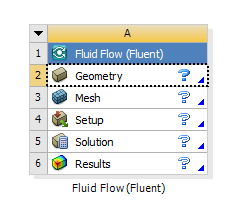
\includegraphics[width=0.4\textwidth]{1.png}
	\caption{Definiciones necesarias para realizar el cálculo.}
\end{figure}

Este recuadro tiene todas las definiciones que necesita para poder proceder a realizar el cálculo del movimiento del fluido. Como primer instancia se encuentra el tipo de proyecto, en este caso es $Fluid Flowe (Fluent)$, posteriormente debemos definir la geometría. Esto es sencillo debido a que ya hemos hecho el modelo que ha definido nuestro sistema a calcular, por lo que sólo habrá que cargarlo al programa directamente. Una vez definida la geometría procederemos a definir la malla, para esto utilizaremos Meshing.

Al abrir la geometría en Meshing habrá distintas opciones, la de mayor interés será la de $Mesh$ donde insertaremos un nuevo método.


\begin{figure}[H]
	\centering
	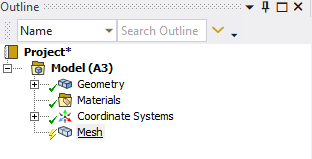
\includegraphics[width=0.4\textwidth]{2.png}
	\caption{Opciones del mallado.}
\end{figure}

Este nuevo método nos permitirá definir las características principales de la malla. De entrada modificaremos el tamaño del elemento a $2 \times 10^{-3} \ m$, y nos aseguraremos de seleccionar la geometría y cambiar el método de cuadriláteros a triángulos.

\begin{figure}[H]
	\centering
	\begin{subfigure}[b]{0.49\linewidth}
		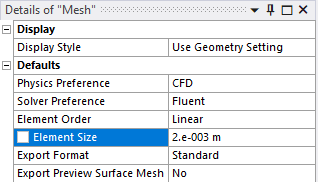
\includegraphics[width=\linewidth]{3.png}
		\caption{Tamaño del elemento.}
	\end{subfigure}
	\begin{subfigure}[b]{0.49\linewidth}
		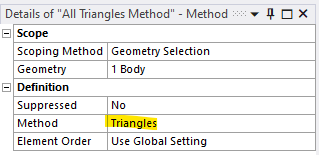
\includegraphics[width=\linewidth]{6.png}
		\caption{Geometría y tipo de método elegido.}
	\end{subfigure}
	\caption{Definición de las propiedades básicas de la malla.}
\end{figure}

Una vez hecho esto, es necesario dar más detalles a los lugares de interés, por lo que crearemos un método de inflación para este objetivo. Primeramente tenemos que definirilo, por lo que lo seleccionamios y debemos de especificar la cara y las fronteras con las que trabajaremos dentro de Meshing.

\begin{figure}[H]
	\centering
	\begin{subfigure}[b]{0.49\linewidth}
		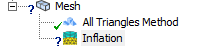
\includegraphics[width=\linewidth]{7.png}
		\caption{Inserción del método de inflación.}
	\end{subfigure}
	\begin{subfigure}[b]{0.49\linewidth}
		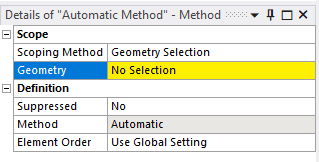
\includegraphics[width=\linewidth]{4.png}
		\caption{Selección de la herramienta de cara.}
	\end{subfigure}
	\caption{La cara a definir es la del modelo, se está trabajando en un análisis bidimensional, sin embargo esta es la herramienta que se utiliza..}
\end{figure}


\begin{figure}[H]
	\centering
	\begin{subfigure}[b]{0.49\linewidth}
		
\includegraphics[width=\linewidth]{9.png}
		\caption{Selección de la cara y las fronteras.}
	\end{subfigure}
	\begin{subfigure}[b]{0.49\linewidth}
		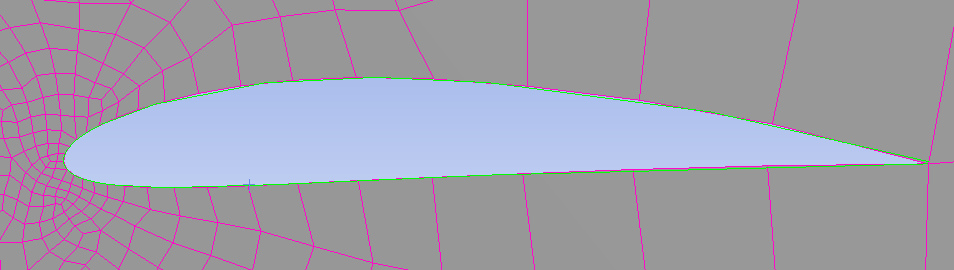
\includegraphics[width=\linewidth]{10.png}
		\caption{Fronteras del perfil alar seleccionadas..}
	\end{subfigure}
	\caption{Definición de las fronteras a inflar.}
\end{figure}

Como último punto antes de dejar listo el método de inflación, es que el número de capas máximas debe de ser de 10, para mejorar los cálculos alrededor de las fronteras.

\begin{figure}[H]
	\centering
	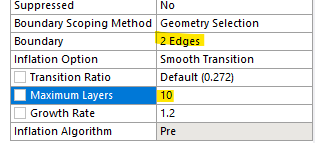
\includegraphics[width=0.4\textwidth]{11.png}
	\caption{Últimas definiciones hechas.}
\end{figure}

Este procedimiento de inflación también se debe aplicar a las fronteras superiores e inferiores del túnel de viento ya que será necesario para el cálculo posteriormente.


El siguiente paso sería definir el número de divisiones al perfil alar. Para realizar esto es necesario definir otro método llamado $sizing$. Para esto procedemos de la misma manera que en las otras ocasiones. Se nos anexará el siguiente recuadro y debemos de elegir las fronteras del álabe, que se modificaran cuando las definamos.

\begin{figure}[H]
	\centering
	\begin{subfigure}[b]{0.49\linewidth}
		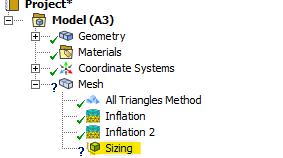
\includegraphics[width=\linewidth]{12.png}
		\caption{Adición del nuevo método.}
	\end{subfigure}
	\begin{subfigure}[b]{0.49\linewidth}
		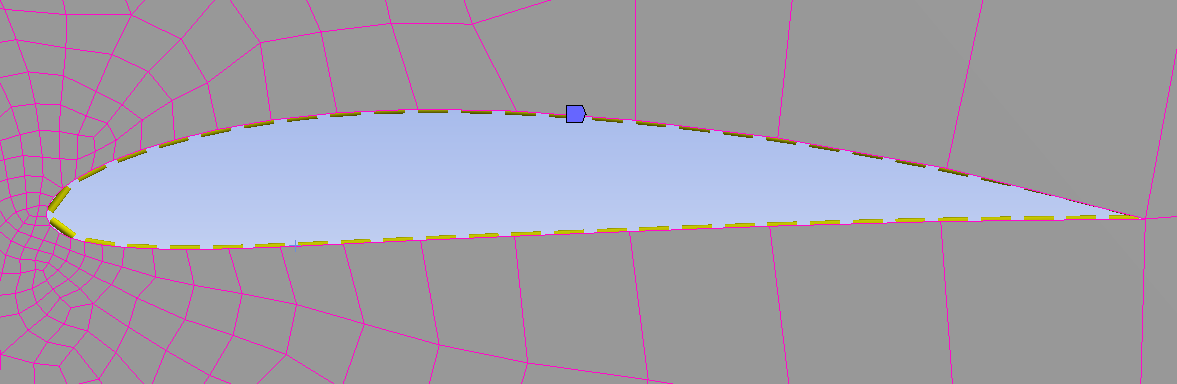
\includegraphics[width=\linewidth]{13.png}
		\caption{Modificación del aspecto del álabe, simbolizando las divisiones.}
	\end{subfigure}
	\caption{Definición del sizing sobre la geometría dada.}
\end{figure}

También es necesario aumentar el número de divisiones como se muestra a continuación.

\begin{figure}[H]
	\centering
	\begin{subfigure}[b]{0.49\linewidth}
		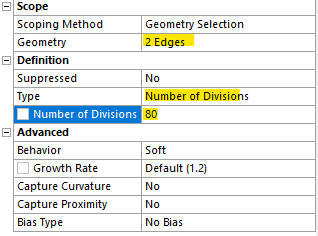
\includegraphics[width=\linewidth]{14.png}
		\caption{Cambio en los parámetros del sizing.}
	\end{subfigure}
	\begin{subfigure}[b]{0.49\linewidth}
		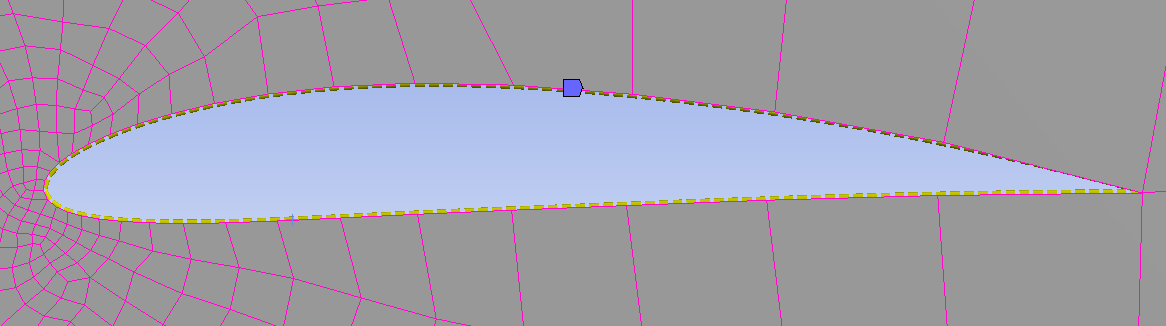
\includegraphics[width=\linewidth]{15.png}
		\caption{Cambio en el aspecto del álabe.}
	\end{subfigure}
	\caption{División del álabe terminada con ochenta nodos a lo largo del perfil.}
\end{figure}

Este aumento en el número de nodos mejora la calidad de la malla. Por último es necesario darle un nombre a cada parte de la geometría. Las geometrías nombradas son la entrada, la salida, la pared superior y la pared inferior del túnel de viento; la frontera superior del álabe, la frontera inferior del álabe y la región en su totalidad.

\begin{figure}[H]
	\centering
	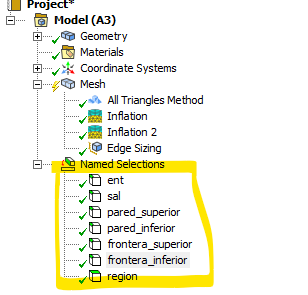
\includegraphics[width=0.5\textwidth]{16.png}
	\caption{Nombramiento de todas las partes de la geomtería.}
\end{figure}


\begin{figure}[H]
	\centering
	\begin{subfigure}[b]{0.49\linewidth}
		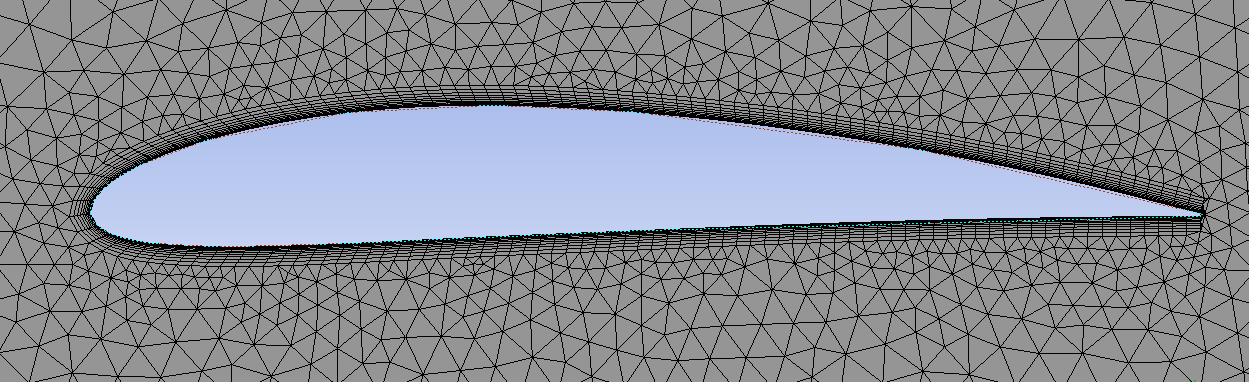
\includegraphics[width=\linewidth]{18.png}
		\caption{Frontera del álabe.}
	\end{subfigure}
	\begin{subfigure}[b]{0.49\linewidth}
		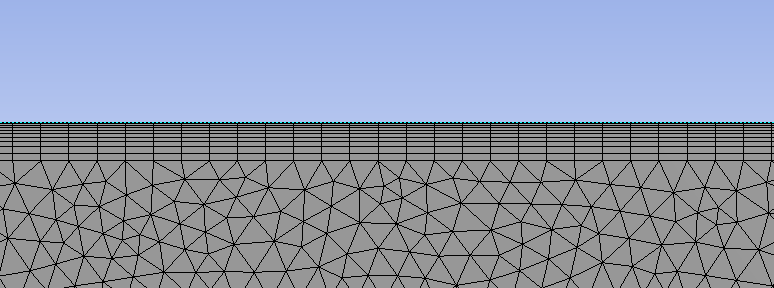
\includegraphics[width=\linewidth]{19.png}
		\caption{Pared superior.}
	\end{subfigure}
	\caption{Detalles en las capas de las fronteras del álabe y la pared superior.}
\end{figure}

\begin{figure}[H]
	\centering
	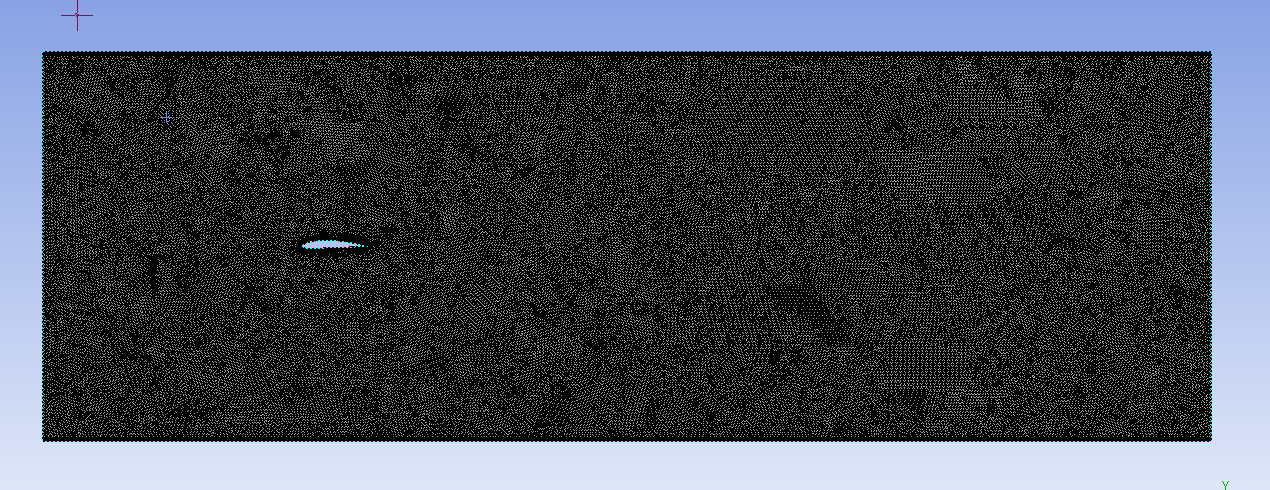
\includegraphics[width=\textwidth]{17.png}
	\caption{Malla definida.}
\end{figure}

\section*{Conclusión}

El procedimieno de mallado es uno de los más importantes en el análisis computacional de dinámica de fluidos, nos determinará gran parte de los resultados, la eficiencia al momento de calcularlos y la precisión de los datos obtenidos. Podemos observar que es un procedimiento sencillo para un perfil alar en dos dimensiones ya que la estructura no presenta gran complejidad, sin embargo cuando se trata de polígonos más complejos o de estructuras tridimensionales fuera de sólidos platónicos o geometrías bien conocidas, la aproximación a éstos objetos se vuelve más y más importante para el cálculo del comportamiendo de los fluidos alrededor o dentro de ellos.

El caso del perfil alar bidimensional nos trae conceptos básicos del mallado y nos permite familiarizarnos con el programa en general para después realizar proyectos más detallados. 

%%%%%  Bib
\renewcommand\refname{References}
\printbibliography
\end{document}
